\chapter{INTRODUCTION}

\section{Overall structure}

- thesis.tex: The main LaTeX document. Compile this file to generate the PDF of your dissertation.

- references.bib: The bibliography file that stores the BibTeX entries of your referenced literature.

- chapters/: A directory containing individual .tex files for each of your thesis chapters. Please replace the placeholder content with your own chapters. Ensure that all figures are correctly referenced.

- figs/: A directory for storing your figure files. It is recommended to organize figures by chapter.

- appendix/: This folder contains supplementary materials, organized by chapter.

\section{Citation}

For citations, please use \verb|\cite{}| or \verb|\citeA{}| to reference literature included in your BibTeX file (e.g., references.bib). For example, global warming has led to widespread lake ice loss over the past century \cite{Huang2022Oct, Sharma2019Mar}. \citeA{He2025Jun} used an LSTM model to simulate daily lake ice cover in the Northern Hemisphere.

\section{Cross reference}

For cross-referencing figures and tables, this template uses the cleveref package, which allows you to reference figures, tables, and sections using \verb|\cref{label}|. For example, \cref{iceloss} shows changes in lake ice intermittency over the past four decades in the Northern Hemisphere; \cref{inputtable} lists the input and output variable of the lake ice model.

\begin{figure}[ht]
\centering
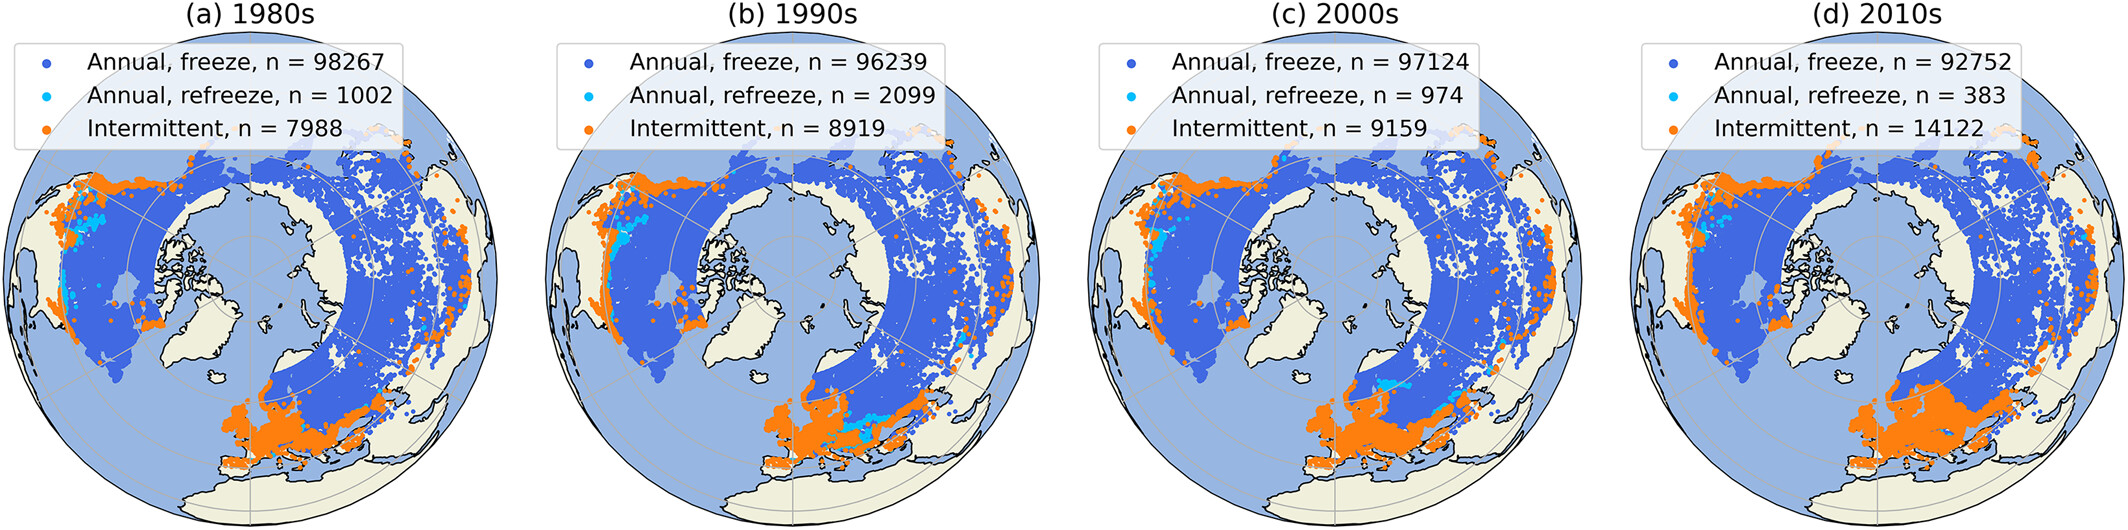
\includegraphics[width=\textwidth]{figs/ch1/iceloss.jpg}
\caption{Geographic distribution of lake ice intermittency over the past four decades. "Annual, refreeze" represents the annually ice-covered lakes which experienced multiple freeze-thaw events during the decade, while the "Annual, freeze" lakes did not experience multiple freeze-thaw events.}
\label{iceloss}
\end{figure}

\begin{table}[ht]
\caption{Summary of the input and output variables for the Long Short Term Memory (LSTM) lake ice cover model. $K$ = Kelvin, $J$ = Joule, $mcm$ = million cubic meters},
\resizebox{\linewidth}{!}{
\begin{tabular}{cccc}
\hline
Group & Variable Name & Description & Unit \\
\hline
Output & Ice Cover & The ratio of ice covered area and total lake surface area & \textbackslash{} \\
Input: Forcings & t2max & daily maximum air temperature at 2 meters above the earth surface & $K$ \\
 & t2min & Daily minimum air temperature at 2 meters above the earth surface & $K$ \\
 & srad & Daily averaged solar radiation downward to the earth surface & $J/m^2$ \\
 & u10 & Eastward windspeed at 10 meters above the earth surface & $m/s$ \\
 & v10 & Northward windspeed at 10 meters above the earth surface & $m/s$ \\
 & tp & Total precipitation & $m$ \\
Input: Lake attributes & Lake\textunderscore area & Lake surface area & $km$ \\
 & Vol\textunderscore total & Total lake or reservoir volume & $mcm$ \\
 & Shore\textunderscore len & Shoreline length & $km$ \\
 & Res\textunderscore time & Average residence time of the lake water & $days$ \\
 & Elevation & Elevation of lake surface & $m$\\
\hline
\end{tabular}
}
\label{inputtable}
\end{table}